\chapter{Một số bài toán ứng dụng}
\label{ch:05}

Trong chương này, ta sẽ cùng nhau giải quyết
hai bài toán học tăng cường cơ bản để minh họa cho việc
sử dụng thuật toán Q-Learning đã được trình bày ở chương trước.
Bài toán đầu tiên sẽ là bài Chiếc taxi thông minh (Smart Taxi);
trong bài toán này, ta sẽ huấn luyện một chiếc taxi
sao cho nó có thể đón và trả khách tại đúng vị trí
và thực hiện việc này một cách "thông minh" nhất có thể.
Bài toán thứ hai sẽ giải quyết việc điều khiển
chiếc xe đẩy để giữ cho con lắc được gắn trên xe
luôn ở trạng thái cân bằng; bài toán kinh điển này còn
được biết đến với cái tên Bài toán cân bằng con lắc ngược (CartPole).

\section{Bài toán chiếc taxi thông minh}
\subsection{Bài toán}
Ta có một chiếc taxi được trang bị các cảm biến, trí tuệ nhân tạo,~\dots\space
để có thể tự vận hành trong mọi điều kiện giao thông và thời tiết.
Nhiệm vụ của chiếc xe này là đón và trả khách tại những vị trí nhất định.
Ngoài ra, việc vận chuyển hành khách cần phải thỏa mãn những tiêu chí sau:
\begin{itemize}
    \item Phải trả khách tại đúng vị trí được chỉ định
    \item Tiết kiệm thời gian cho hành khách một cách tối đa
    \item Đảm bảo hành khách được an toàn và phải tuân thủ tất cả các luật giao thông được đưa ra
\end{itemize}

\subsection{Mô hình hóa bài toán}
Trước khi có thể sử dụng các kỹ thuật học tăng cường
để huấn luyện cho chiếc taxi (agent của chúng ta)
thực hiện công việc đưa đón khách một cách tự động,
ta cần phải quan tâm đến một vài khía cạnh
về việc mô hình hóa bài toán.
Ta cần phải biết phần thưởng (rewards),
không gian trạng thái (state space) của chiếc taxi,
và các hành động (actions) mà chiếc taxi
có thể thực hiện tại mỗi trạng thái.

\subsubsection{Phần thưởng}
Vì chiếc taxi sẽ được huấn luyện bằng cách
thử và sai khi tương tác với môi trường,
ta cần phải định nghĩa phần thưởng và/hoặc hình phạt cho nó:
\begin{itemize}
    \item Chiếc taxi (agent) sẽ nhận được một phần thưởng lớn (+20 điểm)
    khi trả khách thành công (trả đúng vị trí được đưa ra)
    \item Chiếc taxi sẽ bị phạt nặng nếu nó trả khách sai vị trí (-10 điểm)
    \item Chiếc taxi sẽ bị phạt "nhẹ" (slight negative reward)
    trong suốt chuyến hành trình đi đến vị trí trả khách (-1 điểm/bước).
    Hình phạt ở đây không được lớn vì ta không muốn
    việc chiếc taxi cố gắng "lao" đến đích một cách nhanh nhất có thể
    mà vi phạm luật giao thông hay gây nguy hiểm cho hành khách.
\end{itemize}

\subsubsection{Không gian trạng thái}
Không gian trạng thái là tập chứa tất cả những tình huống
mà chiếc taxi của chúng ta có thể gặp phải.
Đây là nơi chứa những thông tin vô cùng cần thiết
cho chiếc taxi để giúp nó có thể đưa ra những hành động "đúng"
tương ứng với trạng thái mà nó đang ở.

Giả sử, ta có một bãi tập cho chiếc taxi của chúng ta,
như được minh họa trong Hình~\ref{fig:training_area};
ở đây, ta sẽ dạy chiếc taxi vận chuyển hành khách
đến các vị trí (R, G, Y, B) trên bãi tập.
\begin{figure}[H]
    \centering
    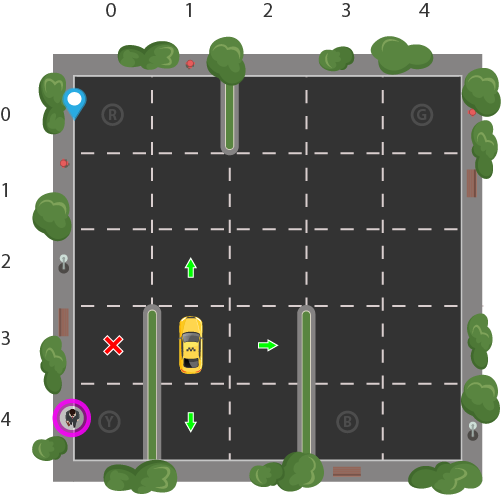
\includegraphics[scale=0.6]{rl_smart_taxi_env.png}
    \caption{Bãi tập.}
    \label{fig:training_area}
\end{figure}

Để đơn giản hóa bài toán, ta có một số giả định như sau:
\begin{itemize}
    \item Chiếc taxi là phương tiện duy nhất có trên bãi tập
    \item Khu vực huấn luyện có thể được chia thành một lưới $5 \times 5$,
    cho ta tổng cộng 25 vị trí mà chiếc taxi có thể đỗ.
    Ví dụ, như ta có thể thấy trên Hình~\ref{fig:training_area},
    chiếc taxi đang nằm tại vị trí có tọa độ (3, 1);
    ngoài ra 4 vị trí R, G, Y, B có tọa độ lần lượt là
    (0,0), (0,4), (4,0), (4,3);
    vị hành khách đáng kính đang đứng tại vị trí Y
    và có mong muốn di chuyển đến vị trí R trên bãi tập.
\end{itemize}

Vậy, ta có tổng cộng $5 \times 5=25$ vị trí mà chiếc taxi có thể xuất hiện,
4 đích đến, và 5 vị trí của hành khách
(4 vị trí tại R, G, Y, B và 1 vị trí là ở trên chiếc taxi).
Tổng số trạng thái có thể có của môi trường sẽ là
$5 \times 5 \times 5 \times 4=500$ trạng thái.

\subsubsection{Không gian hành động}
Tại mỗi thời điểm, chiếc taxi (agent của bài toán)
sẽ nằm ở 1 trong tổng 500 trạng thái,
và nó sẽ thực hiện một hành động tương ứng với trạng thái hiện có.
Hành động ở đây có thể là đón/trả khách, và di chuyển quanh bãi tập.

Không gian hành động của ta sẽ gồm:
\begin{itemize}
    \item Đi lên
    \item Đi xuống
    \item Đi sang trái
    \item Đi sang phải
    \item Đón khách
    \item Trả khách
\end{itemize}

Để ý rằng, tại một số trạng thái ta không thể thực hiện
một vài hành động nhất định.
Ví dụ như khi chiếc taxi ở vị trí mép tường bên trái,
nó không thể thực hiện hành động đi sang trái;
ta có thể giải quyết vấn đề này bằng việc phạt chiếc taxi
khi rơi vào tình huống đó (tình huống bị "đâm" và tường)
và giữ nguyên vị trí hiện tại của nó.

\subsection{Giải quyết bài toán}
Giải pháp được sử dụng để giải quyết bài toán này
sẽ là giải thuật Q-Learning.
Môi trường của bài toán sẽ được mô phỏng nhờ vào sự trợ giúp
của thư viện Gym được cung cấp bởi OpenAI.

Chiếc taxi sẽ được huấn luyện trong 100000 episode
thông qua việc tương tác với môi trường.
Một vài kết quả trong quá trình huấn luyện được minh họa như trong
Hình~\ref{fig:training_episode_step},
\ref{fig:training_episode_penalty} và \ref{fig:training_episode_reward}.

\begin{figure}[H]
    \centering
    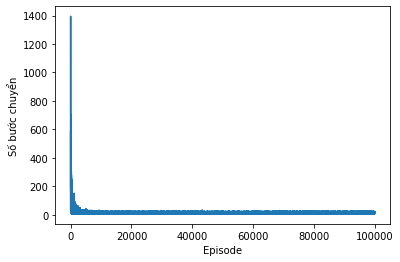
\includegraphics[scale=0.7]{training_episode_step.png}
    \caption{Số bước chuyển chiếc taxi thực hiện tại mỗi episode.}
    \label{fig:training_episode_step}
\end{figure}
\begin{figure}[H]
    \centering
    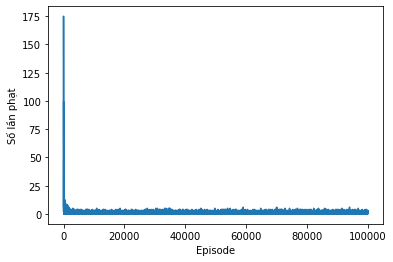
\includegraphics[scale=0.7]{training_episode_penalty.png}
    \caption{Số lần chiếc taxi đón/trả khách sai vị trí tại mỗi episode.}
    \label{fig:training_episode_penalty}
\end{figure}
\begin{figure}[H]
    \centering
    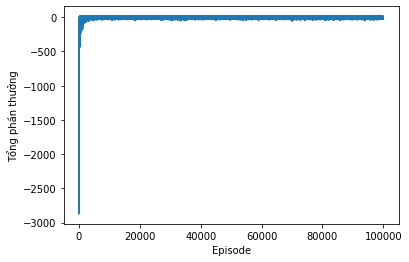
\includegraphics[scale=0.7]{training_episode_reward.png}
    \caption{Số phần thưởng chiếc taxi nhận được tại mỗi episode.}
    \label{fig:training_episode_reward}
\end{figure}

Kết quả chạy của bài toán với 1000 episode
sau quá trình huấn luyện được minh họa như trong Hình~\ref{fig:prediction_results}

\begin{figure}[H]
    \centering
    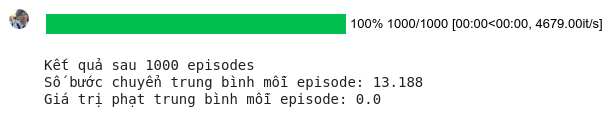
\includegraphics[scale=0.7]{prediction_results.png}
    \caption{Kết quả chạy với 1000 episode.}
    \label{fig:prediction_results}
\end{figure}

Có thể thấy chiếc taxi đã được huấn luyện khá tốt,
không mắc bất cứ sai lầm nào trong việc đón/trả khách
và thực hiện việc chọn đường đi khá "thông minh".


\section{Bài toán cân bằng con lắc ngược}

\begin{figure}[H]
    \centering
    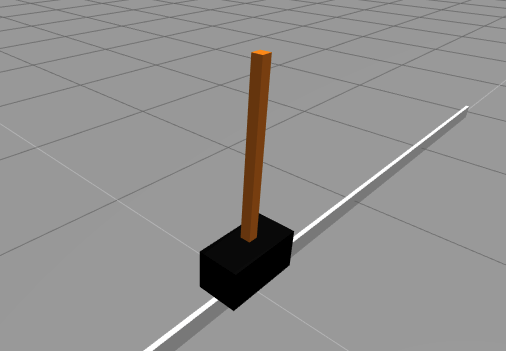
\includegraphics[scale=0.7]{cartpole.png}
    \caption{Hình minh họa bài toán cân bằng con lắc ngược.}
    \label{fig:cartpole}
\end{figure}

\subsection{Bài toán}
Ta có một con lắc ngược được gắn phía trên
một chiếc xe đẩy bằng một khớp nối có thể quay.
Chiếc xe được đặt trên một đường ray không có ma sát
và chỉ có thể di chuyển sang trái hoặc sang phải.
Ở trạng thái khởi đầu, con lắc được đặt thẳng đứng,
hay nói cách khác con lắc và đường thẳng vuông góc
với đường ray tạo thành một góc 0\degree.
Mục tiêu của bài toán là không để cho con lắc bị đổ
bằng cách tăng hoặc giảm vận tốc của xe đẩy.
Trò chơi sẽ kết thúc khi:
\begin{itemize}
    \item con lắc bị "đổ"
    (góc của con lắc nhỏ hơn -12\degree hoặc lớn hơn 12\degree),
    \item hoặc vị trí của xe đẩy năm ngoài đoạn $[-2.4, 2.4]$
    (tâm của chiếc xe đẩy đi ra ngoài khung nhìn),
    \item hoặc số bước vượt quá 200.
\end{itemize}

\subsection{Mô hình hóa bài toán}
\subsubsection{Phần thưởng}
Hệ chuyển động sẽ nhận được phần thưởng +1 sau mỗi bước
(bao gồm cả bước kết thúc).

\subsubsection{Không gian trạng thái}
Mỗi trạng thái của hệ sẽ được cấu tạo bởi 4 thành phần:
\begin{itemize}
    \item Vị trí xe đẩy
    \item Vận tốc xe đẩy
    \item Góc của con lắc ngược
    \item Vận tốc ở đỉnh con lắc
\end{itemize}

Miền giá trị của các thành phần này được minh họa như trong Bảng~\ref{tab:states}.

\begin{table}[H]
    \centering
    \begin{tabular}{|l|l|l|l|}
    \hline
    \multicolumn{1}{|c|}{Chỉ số} & \multicolumn{1}{c|}{Trạng thái} & \multicolumn{1}{c|}{Min} & \multicolumn{1}{c|}{Max} \\ \hline
    0                            & Vị trí xe đẩy                   & -2.4                     & 2.4                      \\ \hline
    1                            & Vận tốc xe đẩy                  & -Inf                     & Inf                      \\ \hline
    2                            & Góc của con lắc ngược           & $\sim$-41.8\degree       & $\sim$41.8\degree        \\ \hline
    3                            & Vận tốc ở đỉnh con lắc          & -Inf                     & Inf                      \\ \hline
    \end{tabular}
    \caption{Các trạng thái của hệ.}
    \label{tab:states}
\end{table}

\subsubsection{Không gian hành động}
Có tổng cộng 2 hành động để di chuyển con lắc,
đó là đẩy xe sang trái và sang phải.

\subsection{Giải quyết bài toán}
Với số trạng thái quá lớn, việc sử dụng giải thuật Q-Learning
như trong bài toán "Chiếc taxi thông minh" trước đó trở nên
bất khả thi về không gian lưu trữ.
Việc sử dụng một mạng nơ-ron nhân tạo (Artificial Neural Network)
thay thế cho bảng Q-Table có vẻ phù hợp hơn rất nhiều.

Hệ xe đẩy con lắc sẽ được huấn luyện trong 50000 episode
thông qua việc tương tác với môi trường.
Một vài kết quả trong quá trình huấn luyện được minh họa như trong
Hình~\ref{fig:cartpole_episode_reward} và \ref{fig:cartpole_running_avg_reward}.

\begin{figure}[H]
    \centering
    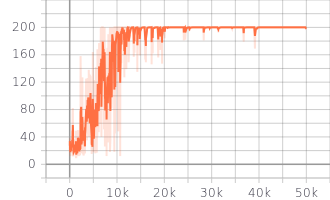
\includegraphics[scale=1]{cartpole_episode_reward.png}
    \caption{Số phần thưởng hệ nhận được tại mỗi episode.}
    \label{fig:cartpole_episode_reward}
\end{figure}

\begin{figure}[H]
    \centering
    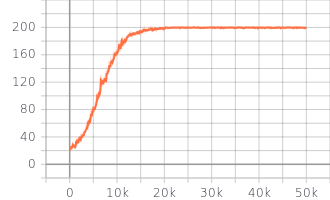
\includegraphics[scale=1]{cartpole_running_avg_reward.png}
    \caption{Số phần thưởng trung bình hệ nhận được qua các episode.}
    \label{fig:cartpole_running_avg_reward}
\end{figure}

Dựa vào các biểu đồ, ta có thể thấy hệ dễ dàng đạt được
số điểm tối đa, 200 điểm, sau khoảng 10000 episode.